\section{Principiul fundamental al dinamicii}

În mecanica newtoniană, legea dinamicii:
\[ m\vec{a} = m\diff{\vec{v}}{t} = \vec{F} \]
are aceeași formă în orice SRI. De aici rezultă că dacă asupra unui corp se
acționează cu o forță constantă un timp îndelungat, viteza acestuia poate
crește oricât de mult.

Teoria relativității einsteiniene implică o schimbare fundamentală și în
dinamică. Postulatul doi al lui Einstein afirmă că viteza limită a corpurilor
sau a câmpurilor electromagnetice este viteza de propagare a luminii în vid:
\( c = 299792458 ~ \mathrm{m/s} \).
Înseamnă că legea dinamicii newtoniene nu mai este valabilă pentru viteze mari
ale corpurilor.

La baza dinamicii relativiste se află legea fundamentală a mecanicii newtoniene,
scrisă sub forma:
\[ \diff{\vec{p}}{t} = \vec{F} \]

În relația de definiție a impulsului \( \vec{p} = m\vec{v} \), masa $m$ nu mai
este un factor de proporționalitate constant între impuls și viteză, ci depinde
de viteza corpului.

Pentru a stabili dependența masei inerte în raport cu viteza corpului, vom folosi
formulele relativiste de compunere a vitezelor și legea conservării impulsului.

\parbreak

\begin{wrapfigure}{r}{0.4\textwidth}
    \centering
    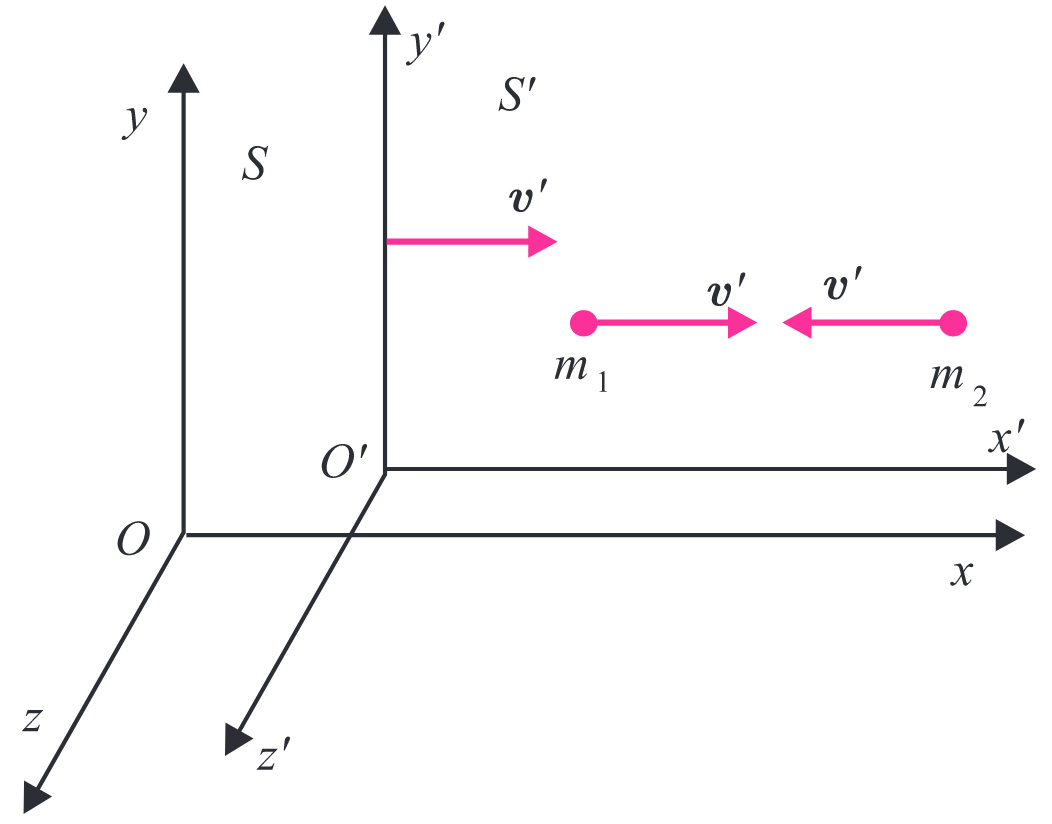
\includegraphics[width=0.4\textwidth]{fig/ciocnire}
    \caption{Ciocnirea inelastică a două corpuri în raport cu S și S'}
\end{wrapfigure}

Considerăm o ciocnire inelastică în raport cu un referențial $S$ și un
referențial $S'$, aflat în mișcare față de $S$ cu viteza $v'$. Cele două
corpuri au aceeași masă, $m_0$, atunci când se află în repaus față de $S$, iar în
referențialul $S'$ se deplasează unul spre celălalt cu vitezele $v'$. În
procesul ciocnirii masa \( m = m_1 + m_2 \) se conservă, iar după ciocnire
se vor afla în repaus față de $S'$ și se vor deplasa cu viteza $v'$ față de
$S$.

Conform formulelor de compunere a vitezelor, avem:
\begin{equation*}
    \begin{aligned}[t]
        v_1 = \frac{v' + v'}{1 + \frac{v'}{c^2}v'} = \frac{2v'}{1 + \frac{v'^2}{c^2}}
    \end{aligned}
    \qquad
    \begin{aligned}[t]
        v_2 = \frac{v' - v'}{1 + \frac{v'}{c^2}v'} = 0
    \end{aligned}
\end{equation*}

\clearpage

Înlocuind în legea conservării impulsului în raport cu $S$:
\[ m_1 v_1 + m_2 v_2 = (m_1 + m_2) v' \]
rezultă:
\[
    \begin{aligned}
        m_1 \frac{2v'}{1 + \frac{v'^2}{c^2}} &= \left( m_1 + m_2 \right)v' \\
        m_1 \left( \frac{2}{1 + \frac{v'^2}{c^2}} - 1 \right) &= m_2
    \end{aligned}
\]

Din \( v_2 = 0 \) rezultă că cel de-al doilea corp se află în repaus față de $S$.
Înseamnă că \( m_2 = m_0 \), și putem afla $m_1$ în funcție de $m_0$:
\[ m_0 = m_1 \frac{1 - \frac{v'^2}{c^2}}{1 + \frac{v'^2}{c^2}} \]

Folosind ecuația:
\[
    1 - \frac{v_1^2}{c^2}
    = 1 - \frac{1}{c^2}\cdot\frac{4v'^2}{\left(1 + \frac{v'^2}{c^2}\right)}
    = \left(\frac{1 - \frac{v'^2}{c^2}}{1 + \frac{v'^2}{c^2}}\right)
\]

\begin{wrapfigure}{r}{0pt}
    \begin{tikzpicture}[scale=0.8]
        \pgfmathsetmacro{\c}{299 792 458}
        \begin{axis}[
            width=6.5cm,
            height=8cm,
            xlabel=$v$,
            ylabel=$m$,
            samples=100,
            ymax=8.5,
            xtick={\c/2,\c},
            ytick={1,2,...,8},
            xticklabels={$0.5c$,$c$},
            yticklabels={$m_0$,$2m_0$,$3m_0$,$4m_0$,$5m_0$,$6m_0$,$7m_0$,$8m_0$},
        ]
            \addplot [domain=0:\c] {1 / sqrt(1 - x^2 / \c^2)};
            \addplot [Asymptote] coordinates {(\c, 0) (\c, 9)};
        \end{axis}
        \node [Origin] {$O$};
    \end{tikzpicture}
    \caption{Dependența $m = f(v)$.}
\end{wrapfigure}

se obține:
\[
    \begin{aligned}
        m_0 &= m_1\sqrt{1 - \frac{v_1^2}{c^2}} \\
        m_1 &= \frac{m_0}{\sqrt{1 - \frac{v_1^2}{c^2}}}
    \end{aligned}
\]

Așadar, dacă un corp are \emph{masa de repaus} $m_0$, atunci când se deplasează cu
viteza $v$ va avea masa:
{
    \color{\accentcolor}
    \[ m = \frac{m_0}{\lorentzradical} \]
}

Pentru \( \frac{v}{c} \rightarrow 0 \), rezultă \( m \rightarrow m_0 \), adică, în
aproximația newtoniană, masa $m$ poate fi confundată cu masa de repaus $m_0$.
